\documentclass[11pt,a4paper]{article}

\usepackage[utf8]{inputenc}
\usepackage[T5]{fontenc}
\usepackage[english,vietnamese]{babel}
\usepackage{mathptmx}
\usepackage[a4paper,margin=22mm]{geometry}
\usepackage{amsmath}
\usepackage{amssymb}
\usepackage{array}
\usepackage{booktabs}
\usepackage{caption}
\usepackage{enumitem}
\usepackage{float}
\usepackage{graphicx}
\usepackage[unicode]{hyperref}
\usepackage{longtable}
\usepackage{makecell}
\usepackage{pdflscape}
\usepackage{tabularx}
\usepackage{xcolor}

\AtBeginDocument{\selectlanguage{vietnamese}}
\hypersetup{
  colorlinks=true,
  linkcolor=blue!45!black,
  urlcolor=blue!45!black,
  citecolor=blue!45!black,
  pdftitle={Gaussian Mixture Source Modeling and Routing for Flow Matching},
  pdfauthor={Kieu Son Tung},
  pdfsubject={IT3930E -- Project II},
  pdfkeywords={flow matching, Gaussian mixture models, learned routing, latent generative modeling}
}

\setlist[itemize]{leftmargin=*,nosep}
\setlist[enumerate]{leftmargin=*,nosep}
\setlength{\parskip}{0.45em}
\setlength{\parindent}{0pt}
\renewcommand{\arraystretch}{1.14}

\newcommand{\fid}{\mathrm{FID}}
\newcommand{\kl}{D_{\mathrm{KL}}}
\newcommand{\stopgrad}{\operatorname{stopgrad}}
\newcommand{\run}[1]{{\small\nolinkurl{#1}}}
\newcommand{\metric}[1]{\texttt{\small\detokenize{#1}}}
\newcommand{\best}[1]{\textbf{#1}}
\newcommand{\na}{--}
\newcolumntype{Y}{>{\raggedright\arraybackslash}X}
\newcolumntype{C}[1]{>{\centering\arraybackslash}p{#1}}

\begin{document}

\begin{titlepage}
\begin{center}

\textsc{\large \textcolor{black}{\textbf{HANOI UNIVERSITY OF SCIENCE AND TECHNOLOGY}}}\\[0.5cm]

{\Large \uppercase{School of Information Communication Technology}\\[1cm]}

\includegraphics[scale=0.13]{figures/logo-soict-hust-1.png}\\[1cm]
\textsc{\Large \textbf{Project II report:}}\\[0.2cm]
{\large IT3930E}\\[0.4cm]

\rule{\linewidth}{0.7mm} \\[0.4cm]
{\huge \bfseries\color{black!70!black} Gaussian Mixture Source Modeling and Routing for Flow Matching \\[0.4cm]}
\rule{\linewidth}{0.7mm} \\[1cm]

\color{black!80!black}{\large \textbf{\textit{Supervised by}:}}\\[0.6cm]

\begin{tabular}{l}
\large Prof. Khoat Than \\[0.4cm]
\large M.Sc. Nguyễn Duy Hiệp \\[1cm]
\end{tabular}

\color{black!80!black}{\large \textbf{\textit{Presented by}:}}\\[0.6cm]
\color{black}
\begin{tabular}{l}
\large Kiều Sơn Tùng - 20235571 \\[0.4cm]
\end{tabular}

\vfill

{\large \color{black!80!black}{\textbf{Hanoi - Vietnam}}\\[0.2cm] \color{blue!90!black}2026}

\end{center}
\end{titlepage}
\selectlanguage{english}
\setcounter{page}{2}

\section*{Project Information}

\begin{tabularx}{\linewidth}{@{}p{0.24\linewidth}Y@{}}
\toprule
\textbf{Course} & IT3930E -- Project II\\
\textbf{Project title} & Gaussian Mixture Source Modeling and Routing for
Flow Matching\\
\textbf{Course supervisor} &
\foreignlanguage{vietnamese}{M.Sc. Nguyễn Duy Hiệp}\\
\textbf{Research supervisor} & Prof. Khoat Than\\
\textbf{Enterprise} & None\\
\textbf{Access} & Private\\
\textbf{Keywords} & Flow Matching; Gaussian mixture models; VAE latents;
learned routing; Diffusion Transformer; Fréchet Inception Distance\\
\bottomrule
\end{tabularx}

\subsection*{Project description}

The project studies whether a learned source distribution can improve latent
Flow Matching. A diagonal Gaussian mixture model is fitted to VAE data
latents, and a convolutional router is trained to approximate the mixture
posterior. The router then selects mixture components used to construct source
latents for the transport path. Experiments compare weighted and sampled
top-\(k\) source construction, endpoint-mix and bridge router training, router
capacity and regularization, GMM initialization, and resume strategies. Image
quality is evaluated with FID at matched checkpoints, with repeated
image-generation seeds and multiple GMM fits used to separate evaluation
noise from source-model uncertainty.

The implementation reuses the DiT backbone, data pipeline, and Flow Matching
path of the Shortcut Models repository. It does not optimize the shortcut
bootstrapping objective. For \metric{train_type=gmm-tide}, the desired-step
input is held constant through \metric{ignore_dt=True}, while the target is the
direct velocity between a routed source latent and a data latent.

\newpage

\begin{abstract}
This report analyzes experiments on Gaussian-mixture source modeling and
learned routing for Flow Matching. The implementation is labeled GMM--TIDE in
the repository and run records, but this Project II study uses only the Flow
Matching training path rather than the full shortcut objective. The experiments
were completed through 23 July 2026, and the evidence is organized by algorithm
rather than execution date. The
historical reference uses K16, top-2, soft 0.75, and Dirichlet-512 with a single
\(\fid_{128}=6.969\) measurement. The strongest controlled evidence is a
\(2\times2\) factorial over source construction
(\metric{weighted} versus \metric{sample_topk}) and router training domain
(\metric{mix} versus \metric{bridge}), evaluated at checkpoint 400k over three
GMM randomization seeds and five image-generation seeds per checkpoint.
\metric{sample_topk}+\metric{mix} has the best aggregate mean, \(7.046\), but
the descriptive sample-topk effect has a 95\% \(t\)-interval that crosses zero.
Bridge is unstable across GMM seeds. Within-checkpoint evaluation noise
(sample SD \(0.019\)--\(0.043\)) is much smaller than variation caused by
refitting the GMM/source. Router distillation accuracy, flow curvature,
balanced component usage, and source scale are useful failure diagnostics but
none is a reliable surrogate for FID. No method in this study has yet
established a matched, repeated improvement over the historical reference.
\end{abstract}

\tableofcontents
\newpage

\section{Conceptual Foundations}

\subsection{Images and VAE latent variables}

Training directly on image pixels is expensive because an image has many
spatial values and contains fine-scale details that are not equally useful to
the transport model. The repository first uses a variational autoencoder
(VAE) \cite{kingma2014vae} to map an image \(I\) to a lower-dimensional
latent tensor:
\[
 x_1=E_{\mathrm{VAE}}(I).
\]
The subscript \(1\) denotes the data endpoint of the flow. The generative model
operates in this latent space rather than in pixel space. After sampling, the
final latent is mapped back to an image by
\(\widehat I=D_{\mathrm{VAE}}(\widehat x_1)\). In this project the VAE is a
representation interface; the experiments change the source distribution and
the transport model, not the VAE training objective.

\subsection{Gaussian Mixture Models}

A single Gaussian distribution represents data with one center and one
covariance structure. A Gaussian mixture model (GMM) combines \(K\) Gaussian
components:
\[
 p_{\mathrm{GMM}}(x)
 =\sum_{k=1}^{K}\pi_k\,\mathcal N(x;\mu_k,\Sigma_k),
 \qquad
 \pi_k\ge 0,\quad \sum_{k=1}^{K}\pi_k=1.
\]
Each component has a mixture weight \(\pi_k\), mean \(\mu_k\), and covariance
\(\Sigma_k\). The components can represent distinct regions of the VAE latent
distribution. This implementation uses diagonal covariance, so every latent
coordinate has its own variance but cross-coordinate covariance is omitted.

The posterior responsibility
\[
 q_{\mathrm{GMM}}(k\mid x)
 =
 \frac{\pi_k\mathcal N(x;\mu_k,\Sigma_k)}
 {\sum_j\pi_j\mathcal N(x;\mu_j,\Sigma_j)}
\]
answers a different question from the mixture weight. The weight \(\pi_k\)
describes how common component \(k\) is before observing \(x\), whereas
\(q_{\mathrm{GMM}}(k\mid x)\) measures how well component \(k\) explains a
particular latent. The GMM is fitted before Flow Matching and supplies fixed
component statistics during the main experiments.

\subsection{Neural routing}

Computing the GMM posterior provides a teacher distribution over components.
The router is a convolutional network that predicts
\[
 q_\phi(k\mid x)=\operatorname{softmax}(f_\phi(x))_k
\]
and is trained to approximate that teacher. At source construction time it
ranks components, retains the top-\(k\) set, and either averages component
samples with normalized weights or samples one selected component. The router
is therefore a component-selection mechanism. It is not a semantic image
classifier, and a better posterior-distillation score does not by itself imply
better generated images.

\subsection{Flow Matching}

Flow Matching trains a time-dependent vector field that transports samples
from a source distribution to the data distribution
\cite{lipman2023flow}. For a routed source latent \(x_0\), a data latent
\(x_1\), and \(t\in[0,1]\), this repository uses the nearly linear path
\[
 x_t=\left[1-(1-\epsilon)t\right]x_0+t x_1,
 \qquad \epsilon=10^{-5}.
\]
Its target velocity is constant along each sampled pair:
\[
 v^\star=x_1-(1-\epsilon)x_0.
\]
A neural network \(v_\psi\) learns this velocity by mean-squared regression:
\[
 \mathcal L_{\mathrm{FM}}
 =\mathbb E\!\left[
 \left\|v_\psi(x_t,t,\text{conditioning})-v^\star\right\|_2^2
 \right].
\]
At inference time, numerical integration follows the learned field from a new
source latent toward a generated data latent. The role of the GMM and router is
to change how \(x_0\) and its conditioning statistics are constructed; the
regression target remains a Flow Matching target.

\subsection{DiT backbone and the boundary of this project}

The velocity network is a Diffusion Transformer (DiT), a Transformer that
operates on patches of a latent tensor rather than image pixels
\cite{peebles2023dit}. In the studied path, DiT receives \(x_t\), time \(t\),
the class label, and embeddings of the routed GMM mean and standard deviation.
The component identifier itself is not passed as a separate categorical input.

Shortcut Models extend a flow model by conditioning it on a requested step
size and by constructing bootstrap targets for nonzero shortcut lengths
\cite{frans2024shortcut}. That mechanism is present in the source repository,
but it is outside this Project II experiment. The \metric{gmm-tide} mode sets
\metric{ignore_dt=True}; consequently, the desired-step input is constant and
the update uses the direct Flow Matching target above. “Shortcut Models”
therefore identifies the codebase from which the implementation was reused,
not the title or claimed scope of this project.

\subsection{Fréchet Inception Distance}

Fréchet Inception Distance (FID) compares the means and covariances of
Inception-network features extracted from real and generated image sets
\cite{heusel2017fid}. If their fitted feature distributions have statistics
\((m_r,C_r)\) and \((m_g,C_g)\), then
\[
 \fid
 =\|m_r-m_g\|_2^2
 +\operatorname{Tr}\!\left(
 C_r+C_g-2(C_rC_g)^{1/2}
 \right).
\]
Lower is better under a fixed evaluation protocol. FID evaluates two image
sets, not individual images, and its estimate changes with sample count and
random generation seed. This is why the main comparisons use matched
checkpoints, the same number of generated images, and repeated evaluation
seeds.

\section{Executive Summary}

\subsection{Reference and comparison boundary}

The historical reference is
\run{tide-k16-top2-softv0p75-s128-dir512}:
\[
 K=16,\qquad m=2,\qquad \tau=0.75,\qquad
 \alpha_{\mathrm{Dirichlet}}=512,\qquad \fid_{128}=6.969.
\]
It is a GMM--TIDE run with the same main FM/DiT backbone as the subsequent
ablations. However, \(6.969\) is one historical single-evaluation score at an
unmatched checkpoint. It is therefore a reference line, not an estimate with
the same repeated-evaluation protocol used in the final factorial study.

Three leaderboards must be kept separate:

\begin{center}
\small
\begin{tabularx}{\linewidth}{@{}p{0.23\linewidth}Y c c Y@{}}
\toprule
\textbf{Evidence class} & \textbf{Best observed configuration} &
\textbf{FID128} & \textbf{Step} & \textbf{Interpretation}\\
\midrule
Historical reference & K16/top2/soft0.75/Dirichlet-512 &
6.969 & 365.6k & One unmatched evaluation; not a repeated mean.\\
Exploratory single evaluation & C4, GMM seed 1 &
6.864 & 320k & Best checkpoint selected from a trajectory; selection bias is
possible.\\
Repeated checkpoint, one GMM seed & C4, GMM seed 1 &
6.913 & 400k & Mean over five evaluation seeds, but favorable only for this
GMM initialization.\\
Repeated checkpoint, three GMM seeds & S+M &
\best{7.046} & 400k & Best aggregate in the matched \(2\times2\) factorial;
still above 6.969.\\
\bottomrule
\end{tabularx}
\end{center}

\subsection{Main findings}

\begin{enumerate}
  \item \textbf{Sample-topk is the most promising source change, but the
  evidence is not conclusive.} Across three GMM seeds, its descriptive main
  effect relative to weighted construction is \(-0.117\) FID with sample SD
  \(0.154\); the 95\% \(t\)-interval is \([-0.498,0.265]\).
  \item \textbf{Bridge is not uniformly beneficial.} Its main effect is
  \(+0.086\) FID with sample SD \(0.254\), and it changes from favorable in
  GMM seeds 0--1 to strongly unfavorable in seed 2.
  \item \textbf{GMM randomization dominates image-generation noise.}
  Within a fixed checkpoint, repeated-FID SD is only \(0.019\)--\(0.043\).
  Across GMM fits, both cell rankings and paired effects change materially.
  \item \textbf{Phase-1 accuracy and phase-2 quality are not aligned.}
  Router top-1 agreement or distillation KL can improve while FID worsens.
  The router must approximate the GMM posterior, but that approximation is not
  the downstream objective.
  \item \textbf{Common diagnostics do not rank image quality.} Lower
  curvature, higher usage entropy, source magnitude close to \(x_1\), and
  lower valid loss each fail as standalone FID predictors.
  \item \textbf{The velocity field remains under-dispersed.} Across many
  families, predicted velocity variance is only \(0.63\)--\(0.67\) of target
  velocity variance. Router regularization did not remove this shared failure
  mode.
\end{enumerate}

\section{Algorithm Formulation}

\subsection{Diagonal GMM over data latents}

Let \(x_1\in\mathbb{R}^{H\times W\times C}\) denote a VAE data latent and let
\(\operatorname{vec}(x_1)\in\mathbb{R}^{D}\). The fitted model is a
\emph{diagonal}, not isotropic, Gaussian mixture:
\[
 p_{\mathrm{GMM}}(x)
 =\sum_{k=1}^{K}\pi_k\,\mathcal N(x;\mu_k,\Sigma_k),
 \qquad
 \Sigma_k=\operatorname{diag}(\sigma_{k,1}^{2},\ldots,\sigma_{k,D}^{2}).
\]
An isotropic component would instead use
\(\Sigma_k=s_k^2 I\), one scalar variance shared by all coordinates. Diagonal
covariance permits a different variance per latent coordinate, giving
axis-aligned ellipsoidal rather than spherical contours, while still omitting
off-diagonal correlations.

The component posterior is
\[
 q_{\mathrm{GMM}}(k\mid x)
 =
 \frac{\pi_k\mathcal N(x;\mu_k,\Sigma_k)}
      {\sum_{j=1}^{K}\pi_j\mathcal N(x;\mu_j,\Sigma_j)}.
\]
The GMM parameters \(\pi_k,\mu_k,\Sigma_k\) are learned by diagonal-GMM EM;
they are arrays, not neural-network outputs.

\subsection{Router and distillation objective}

The neural router predicts
\[
 q_\phi(k\mid x)=\operatorname{softmax}(f_\phi(x))_k.
\]
The current architecture is a convolutional trunk followed by global average
pooling and a two-layer MLP:
\[
\begin{aligned}
x
&\longrightarrow
\bigl[\operatorname{Conv}_{3\times3}
\rightarrow\operatorname{Norm?}
\rightarrow\operatorname{SiLU}
\rightarrow\operatorname{Dropout?}\bigr]^d\\
&\longrightarrow\operatorname{GlobalAvgPool}_{H,W}
\rightarrow\operatorname{Dense}_{M}
\rightarrow\operatorname{Norm?}
\rightarrow\operatorname{SiLU}
\rightarrow\operatorname{Dropout?}
\rightarrow\operatorname{Dense}_{K}.
\end{aligned}
\]
Global average pooling averages spatial positions within each feature channel;
it does not average convolution kernels. It trades spatial detail for a fixed
size, translation-tolerant representation.

\begin{figure}[H]
  \centering
  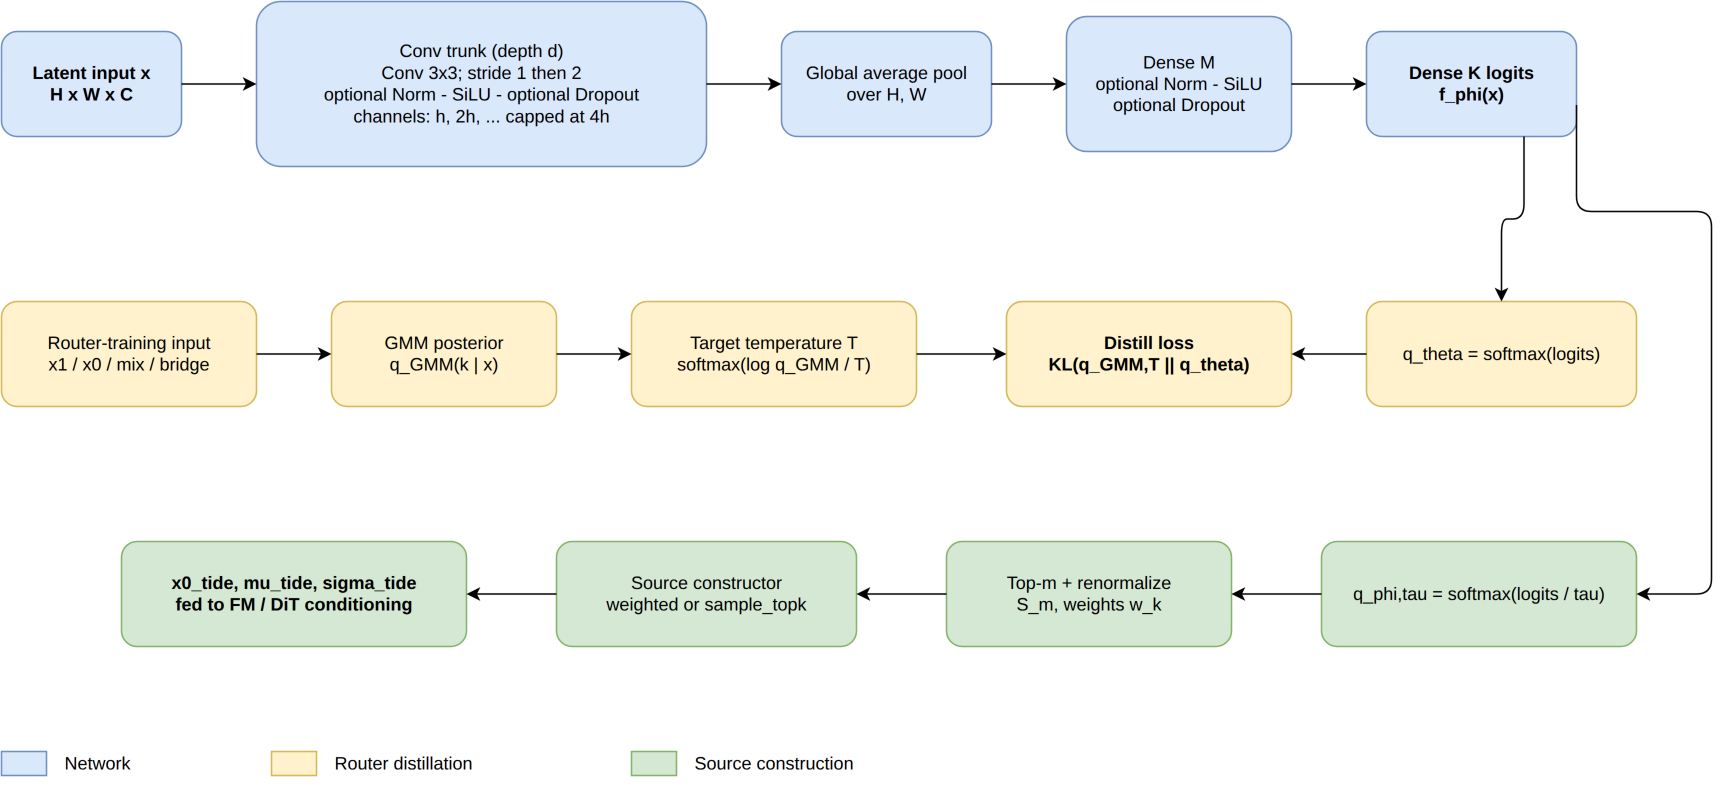
\includegraphics[width=0.99\linewidth]{figures/router_architecture.png}
  \caption{Router architecture and the two uses of its logits. The yellow path
  is GMM-posterior distillation. The green path applies source temperature,
  top-\(m\) routing, and source construction before FM.}
\end{figure}

For soft-KL distillation, target temperature \(T\) is applied to the
\emph{teacher target}:
\[
 \widetilde q_{\mathrm{GMM},T}(k\mid x)
 =
 \frac{q_{\mathrm{GMM}}(k\mid x)^{1/T}}
 {\sum_j q_{\mathrm{GMM}}(j\mid x)^{1/T}},
 \qquad
 \mathcal L_{\mathrm{distill}}
 =\kl\!\left(\widetilde q_{\mathrm{GMM},T}\,\Vert\,q_\phi\right).
\]
Thus \(T>1\) softens the labels used to train the router. This is distinct from
the source temperature \(\tau\), introduced below.

\subsection{Router training domains: data, mix, and bridge}

The router can be distilled on several input domains:
\[
\begin{array}{ll}
\text{\(x_1\)-only:} & x^r=x_1,\\[2mm]
\text{mix:} &
x^r=\begin{cases}x_1,&b=1\\x_0,&b=0,\end{cases}
\quad b\sim\operatorname{Bernoulli}(p),\\[4mm]
\text{bridge:} &
x^r=\lambda x_1+(1-\lambda)x_0,\quad
\lambda\sim\operatorname{Beta}(a,b).
\end{array}
\]
The direct bridge target used here is
\[
 \mathcal L_{\mathrm{bridge}}
 =\kl\!\left(
 q_{\mathrm{GMM}}(\cdot\mid x^r)
 \,\Vert\,
 q_\phi(\cdot\mid x^r)
 \right).
\]
Mix exposes the router to two discrete endpoint domains. Bridge fills the
continuous segment between them and therefore regularizes the input-domain
transition.

Bridge itself does \textbf{not} create an FM gradient path through the router.
It adds distillation supervision at midpoint inputs. If the router is frozen
during FM, bridge affects phase 2 only through the router learned in phase 1.
If joint updates are enabled, the distillation terms update the router; an FM
gradient reaches routing logits only when the route estimator is differentiable
or uses a surrogate such as straight-through or Gumbel-softmax.

\subsection{Source construction}

First sample a base component and latent:
\[
 k_0\sim\operatorname{Categorical}(\pi),\qquad
 x_0^{\mathrm{base}}\sim\mathcal N(\mu_{k_0},\Sigma_{k_0}).
\]
The router produces source probabilities
\[
 q_{\phi,\tau}(k\mid x_0^{\mathrm{base}})
 =
 \operatorname{softmax}\!\left(
 \frac{f_\phi(x_0^{\mathrm{base}})}{\tau}
 \right)_k.
\]
Here \(\tau\) is the \emph{source temperature}; it changes route sharpness
immediately before top-\(m\) selection. Let
\[
 S_m=\operatorname{TopK}_m(q_{\phi,\tau}),\qquad
 w_k=
 \frac{q_{\phi,\tau}(k\mid x_0^{\mathrm{base}})}
 {\sum_{j\in S_m}q_{\phi,\tau}(j\mid x_0^{\mathrm{base}})}
 \quad(k\in S_m).
\]

The main source constructors are:
\[
\begin{aligned}
\text{Weighted (W):}\quad
&z_k\sim\mathcal N(\mu_k,\Sigma_k),\qquad
x_0^{\mathrm{tide}}=\sum_{k\in S_m}w_k z_k,\\
\text{Sample-topk (S):}\quad
&\widetilde k\sim\operatorname{Categorical}(w_{S_m}),\qquad
x_0^{\mathrm{tide}}\sim\mathcal N(\mu_{\widetilde k},\Sigma_{\widetilde k}),\\
\text{Hard top-1:}\quad
&\widehat k=\arg\max_k q_{\phi,\tau}(k\mid x_0^{\mathrm{base}}),\qquad
x_0^{\mathrm{tide}}\sim\mathcal N(\mu_{\widehat k},\Sigma_{\widehat k}).
\end{aligned}
\]
Weighted construction can place the result between components. Sample-topk
selects one component according to relative top-\(m\) strength and preserves
that component's covariance. It is stochastic but is not a uniform draw unless
the selected probabilities are equal.

For weighted construction, the conditioning moments used by the implementation
are
\[
 \mu^{\mathrm{tide}}=\sum_{k\in S_m}w_k\mu_k,\qquad
 (\sigma^{\mathrm{tide}})^2
 =\sum_{k\in S_m}(w_k\sigma_k)^2,
\]
where operations on \(\sigma_k\) are coordinate-wise.

\subsection{Straight-through and Gumbel routing}

A hard top-\(m\) operation is non-differentiable with respect to component
membership. The straight-through estimator uses
\[
 w_{\mathrm{ST}}
 =q_\phi+\stopgrad(w_{\mathrm{hard}}-q_\phi).
\]
The forward pass equals \(w_{\mathrm{hard}}\), while the backward pass uses the
gradient of \(q_\phi\). Gumbel-softmax adds sampled Gumbel noise:
\[
 y_k=
 \frac{\exp((\ell_k+g_k)/\tau_g)}
 {\sum_j\exp((\ell_j+g_j)/\tau_g)},\qquad
 g_k\sim\operatorname{Gumbel}(0,1),
\]
and can be combined with a straight-through hard sample. These methods allow
an approximate FM gradient to routing logits, but they also introduce bias or
variance. Their empirical results did not show an advantage in the tested
regime.

\subsection{Flow Matching objective}

FM uses the pair \((x_0^{\mathrm{tide}},x_1)\):
\[
 x_t=\left[1-(1-\epsilon)t\right]x_0^{\mathrm{tide}}+t x_1,
 \qquad
 v^\star=x_1-(1-\epsilon)x_0^{\mathrm{tide}}.
\]
The DiT predicts
\[
 \mathcal L_{\mathrm{FM}}
 =
 \mathbb E
 \left[
 \left\|
 v_\psi(x_t,t,\Delta t,y,\mu^{\mathrm{tide}},\sigma^{\mathrm{tide}})
 -v^\star
 \right\|_2^2
 \right].
\]
The GMM-derived \(\mu^{\mathrm{tide}}\) and
\(\sigma^{\mathrm{tide}}\) condition the DiT; they are not replacements for
\(x_t\).

\subsection{C0--C5 candidate recipes}

All C0--C5 candidates use K16/top2/soft0.75/Dirichlet-512 and the same DiT/FM
backbone. The identifiers remain fixed across screening, confirmation, resume,
and repeated evaluation; a later C0 or C4 is the same recipe at a different
GMM seed, checkpoint, or evaluation protocol.

\begin{center}
\small
\setlength{\tabcolsep}{4pt}
\begin{tabularx}{\linewidth}{@{}c c c c Y@{}}
\toprule
\textbf{ID} & \textbf{Router data} & \textbf{Source} &
\textbf{Additional change} & \textbf{Purpose}\\
\midrule
C0 & mix (M) & weighted (W) & none &
Matched control for phase-2 source experiments.\\
C1 & bridge (B) & weighted (W) & none &
Isolates bridge relative to C0.\\
C2 & mix (M) & weighted (W) & depth 4, dropout 0.2 &
Isolates router capacity/regularization.\\
C3 & bridge (B) & weighted (W) & depth 4, dropout 0.2 &
Tests bridge with the best local capacity change.\\
C4 & bridge (B) & sample-topk (S) & none &
Changes both the router domain and source constructor.\\
C5 & bridge (B) & weighted (W) & PCA init + 5 Lloyd steps &
Tests a different GMM initialization.\\
\bottomrule
\end{tabularx}
\end{center}

\section{Regularization and Optimization Controls}

\subsection{Network regularization}

\begin{longtable}{@{}p{0.21\linewidth}p{0.73\linewidth}@{}}
\toprule
\textbf{Mechanism} & \textbf{Implementation and intended effect}\\
\midrule
\endhead
Dropout &
Applied after convolutional and MLP activations while training the router.
Disabled during source generation and evaluation. It reduces co-adaptation but
does not directly constrain component usage.\\
\addlinespace
LayerNorm &
Applied at configured convolutional/pooled/MLP locations. It normalizes each
sample's features and stabilizes activation scale. LayerNorm alone was weaker
than the best dropout setting.\\
\addlinespace
GroupNorm &
Normalizes channel groups without batch statistics. It was tested with dropout
0.2 and 0.3 but did not improve over dropout-only.\\
\addlinespace
Weight decay &
Standard parameter shrinkage in the router optimizer. It regularizes weights,
not posterior entropy or component balance.\\
\addlinespace
EMA &
Maintains
\(\phi_{\mathrm{EMA}}\leftarrow\beta\phi_{\mathrm{EMA}}+
(1-\beta)\phi\).
It can stabilize a noisy jointly updated router at evaluation time. The EMA
resume experiment restarted optimizer state and therefore is not a matched
fresh-run comparison.\\
\bottomrule
\end{longtable}

\subsection{Posterior and usage regularization}

\paragraph{Per-sample entropy floor.}
Let
\[
 h(x)=\frac{H(q_\phi(\cdot\mid x))}{\log K}\in[0,1].
\]
The floor penalty is
\[
 \mathcal L_{\mathrm{floor}}
 =
 \mathbb E_x\left[\max(h_0-h(x),0)^2\right].
\]
It activates only when an individual prediction is sharper than the requested
entropy floor. It does not require every component to be used over a batch.

\paragraph{Usage prior near uniform.}
Let the batch-average soft usage be
\[
 \bar q_k=\frac1B\sum_{i=1}^{B}q_\phi(k\mid x_i).
\]
A uniform-usage penalty can be written as
\[
 \mathcal L_{\mathrm{usage}}
 =\kl(\bar q\,\Vert\,u)
 =\sum_k\bar q_k\log(K\bar q_k)
 =\log K-H(\bar q),
\qquad u_k=\frac1K.
\]
This term discourages global batch collapse. It can be small even when each
sample is routed sharply, provided different samples choose different
components.

\paragraph{Entropy reward.}
The joint objective may include
\[
 \mathcal L_{\mathrm{entropy}}
 =-w_H\,\mathbb E_x H(q_\phi(\cdot\mid x)).
\]
Unlike the usage prior, this rewards soft predictions for each sample. It can
blur routing if too strong. Usage balance and per-sample entropy therefore
address different collapse modes.

\paragraph{Tide-KL.}
The additional downstream-domain consistency term is
\[
 \mathcal L_{\mathrm{tide}}
 =
 w_{\mathrm{tide}}\,
 \kl\!\left(
 q_{\mathrm{GMM}}(\cdot\mid x_0^{\mathrm{tide}})
 \,\Vert\,
 q_\phi(\cdot\mid x_0^{\mathrm{tide}})
 \right).
\]
It asks the router to match the GMM posterior on generated source inputs. In
the tested runs it reduced curvature but worsened FID, indicating that
posterior consistency at this domain can be misaligned with image quality.

\section{Metrics and Evidence Protocols}

\subsection{Primary and diagnostic metrics}

\begin{longtable}{@{}p{0.25\linewidth}p{0.69\linewidth}@{}}
\toprule
\textbf{Metric} & \textbf{Definition and interpretation}\\
\midrule
\endhead
FID128 &
Primary ranking metric, evaluated with 128 denoising steps. Lower is better.
FID32 is intentionally omitted from this report.\\
\addlinespace
Router top-1 agreement &
\(\Pr[\arg\max q_\phi=\arg\max q_{\mathrm{GMM}}]\in[0,1]\).
It measures distillation classification agreement, not source quality or FID.\\
\addlinespace
Predicted/target variance ratio &
\[
R_v=\frac{\operatorname{Var}(v_\psi)}
{\operatorname{Var}(v^\star)}.
\]
\(R_v<1\) is called \emph{under-dispersed relative to the FM velocity target}:
the distribution of predicted velocity values has less variance than
\(v^\star=x_1-(1-\epsilon)x_0^{\mathrm{tide}}\). This does not refer to a
``target policy'', and it does not by itself prove mode collapse or angular
error.\\
\addlinespace
Flow curvature proxy &
For normalized rollout segment directions
\(u_r=(x_{r+1}-x_r)/\|x_{r+1}-x_r\|_2\),
\[
\kappa=\frac1{R-1}\sum_r\|u_{r+1}-u_r\|_2\in[0,2].
\]
Zero means consecutive segments are parallel. Lower curvature does not ensure
the correct endpoint distribution.\\
\addlinespace
Router usage entropy &
For hard top-1 batch counts \(p_k=n_k/B\),
\[
H_{\mathrm{use}}=
-\frac{\sum_kp_k\log p_k}{\log K}\in[0,1].
\]
One means uniform component use across the batch; zero means all samples select
one component. This differs from per-sample posterior entropy.\\
\addlinespace
Source magnitude ratio &
\[
R_x=\frac{\mathbb E\|x_0^{\mathrm{tide}}\|_2}
{\mathbb E\|x_1\|_2}.
\]
Values near one rule out a first-order scale mismatch but do not establish
distributional or angular alignment.\\
\addlinespace
Top-k angular dispersion &
\[
D_\angle=
\sum_{k\in S_m}w_k\left[1-\cos(\mu_k,\mu^{\mathrm{tide}})\right]\in[0,2].
\]
It measures directional disagreement among selected centers. Larger values
mean more angular diversity, not necessarily better transport.\\
\addlinespace
Input-domain KL &
\(\kl(q_{\mathrm{GMM}}(\cdot\mid x)\Vert q_\phi(\cdot\mid x))\), evaluated
separately on \(x_0\), midpoint, and \(x_1\). ``KL shift by input domain''
means the router approximates the same teacher with different error depending
on where \(x\) lies along the transport path.\\
\bottomrule
\end{longtable}

\subsection{Evidence hierarchy}

\begin{center}
\small
\begin{tabularx}{\linewidth}{@{}p{0.24\linewidth}c c Y@{}}
\toprule
\textbf{Protocol} & \textbf{Checkpoint control} &
\textbf{Replication} & \textbf{Allowed conclusion}\\
\midrule
Exploratory best checkpoint & No; best step selected &
Usually one GMM fit and one eval & Candidate discovery only.\\
Matched 200k confirmation & Yes; same 200k horizon &
One or two GMM seeds & Short-horizon source diagnostics.\\
Matched 400k repeated-FID & Yes; checkpoint 400k &
3 GMM seeds \(\times\) 5 eval seeds & Main factorial evidence.\\
Historical 6.969 reference & Unmatched &
One reported evaluation & Context only; not a matched control estimate.\\
\bottomrule
\end{tabularx}
\end{center}

The three GMM seeds vary GMM initialization/randomization. They are not fully
independent end-to-end training seeds because router/FM random-number streams
were not independently resampled under a complete seed protocol. Statistical
intervals over \(n=3\) must therefore be interpreted as descriptive
sensitivity, not population-level uncertainty.

\section{Results by Algorithm}

\subsection{All exploratory FID results}

Figure~\ref{fig:landscape} contains all 78 single-evaluation rows in the frozen
plot inventory. The panels are separated by the training step where each best
score was recorded, so a 180k run is not visually ranked as though it shared
the 400k protocol. The dense style is retained to expose the full search
surface; no causal claim is drawn from this figure.

\begin{landscape}
\begin{figure}[H]
  \centering
  \includegraphics[width=0.98\linewidth,height=0.78\textheight,keepaspectratio]{figures/algorithm_fid_landscape.png}
  \caption{Exploratory FID landscape for all 78 single-evaluation records,
  separated into training-step windows. Point color denotes algorithm family.
  The dashed line is the unmatched historical reference.}
  \label{fig:landscape}
\end{figure}
\end{landscape}

\subsection{Router capacity, normalization, dropout, and temperature}

The best local capacity/regularization setting was depth 4 with dropout 0.2.
Increasing depth to 5 or 7 did not continue the trend. Target temperature
softened distillation labels but did not create a monotonic FID improvement.

\begin{figure}[H]
  \centering
  \includegraphics[width=0.92\linewidth]{figures/router_ablation_fid.png}
  \caption{Router regularization, capacity, and target-temperature ablations.
  Values are exploratory best single-evaluation scores; the checkpoint step is
  shown in each label.}
\end{figure}

\begin{center}
\small
\setlength{\tabcolsep}{3pt}
\begin{tabularx}{\linewidth}{@{}Y c c c c c c c@{}}
\toprule
\textbf{Configuration} & \textbf{Depth} & \textbf{FID128} &
\textbf{Step} & \textbf{Top1} & \textbf{\(R_v\)} &
\textbf{Curv.} & \textbf{Usage H}\\
\midrule
dropout 0.2, no norm & 4 & \best{7.094} & 300k & 0.943 & 0.651 & 0.02084 & 0.949\\
LayerNorm + dropout 0.2 & 3 & 7.147 & 350k & 0.912 & 0.669 & 0.02082 & 0.944\\
dropout 0.3, no norm & 3 & 7.153 & 350k & 0.914 & 0.628 & 0.02083 & 0.950\\
LayerNorm + dropout 0.2 & 5 & 7.164 & 300k & 0.964 & 0.661 & 0.02091 & 0.948\\
dropout 0.2, target \(T=1.25\) & 5 & 7.222 & 350k & 0.961 & 0.635 & 0.02080 & 0.950\\
low capacity, plain & 2 & 7.255 & 300k & 0.820 & 0.674 & 0.02072 & 0.940\\
LayerNorm + dropout 0.2 & 7 & 7.282 & 300k & 0.936 & 0.643 & 0.02087 & 0.955\\
GroupNorm + dropout 0.2 & 3 & 7.325 & 250k & 0.914 & 0.633 & 0.02068 & 0.946\\
LayerNorm only & 3 & 7.417 & 300k & 0.907 & 0.650 & 0.02060 & 0.947\\
dropout 0.1, no norm & 3 & 7.422 & 300k & 0.915 & 0.662 & 0.02071 & 0.945\\
\bottomrule
\end{tabularx}
\end{center}

The depth-5 model attains better router top-1 agreement than the depth-4
winner but worse FID. This is direct evidence that router imitation accuracy is
not a downstream ranking metric.

\subsection{Router smoothing and bridge inputs}

\begin{center}
\small
\setlength{\tabcolsep}{3pt}
\begin{tabularx}{\linewidth}{@{}Y c c c c c c@{}}
\toprule
\textbf{Configuration} & \textbf{FID128} & \textbf{Step} &
\textbf{Top1} & \textbf{\(R_v\)} & \textbf{Curv.} &
\textbf{Usage H}\\
\midrule
bridge \(B(1,1)\), FM uniform & \best{7.033} & 350k & 0.907 & 0.672 & 0.02093 & 0.884\\
bridge \(B(2,2)\) & 7.277 & 300k & \na & 0.650 & 0.02088 & 0.939\\
sample-topk + LayerNorm + dropout 0.2 & 7.302 & 300k & \na & 0.656 & 0.02069 & 0.952\\
target \(T=2.0\) & 7.396 & 300k & \na & 0.643 & 0.02086 & 0.939\\
bridge \(B(3,1.4)\), FM uniform & 7.404 & 300k & 0.868 & 0.665 & 0.02062 & 0.864\\
target \(T=1.5\) & 7.506 & 300k & \na & 0.644 & 0.02077 & 0.947\\
entropy floor 0.25, weight 0.05 & 7.533 & 300k & \na & 0.649 & 0.02069 & 0.946\\
bridge \(B(2.2,1.2)\), FM uniform & 7.612 & 300k & 0.888 & 0.660 & 0.02080 & 0.896\\
\bottomrule
\end{tabularx}
\end{center}

Uniform bridge was the best exploratory router-domain change. Endpoint-biased
bridge distributions were worse, suggesting that broad path coverage mattered
more than concentrating router samples near \(x_1\). This observation did not
survive all GMM seeds in the matched factorial, so it remains conditional.

\subsection{Source routing, Gumbel/ST, whitening, and Tide-KL}

\begin{center}
\small
\setlength{\tabcolsep}{3pt}
\begin{tabularx}{\linewidth}{@{}Y c c c c c c@{}}
\toprule
\textbf{Configuration} & \textbf{FID128} & \textbf{Step} &
\textbf{Top1} & \textbf{\(R_v\)} & \textbf{Curv.} &
\textbf{Usage H}\\
\midrule
\(x_1\)-frozen, top2 \(\tau=1.25\), beta(3,1.4) &
\best{7.986} & 180k & \na & 0.637 & \na & \na\\
\(x_1\)-frozen, top4 \(\tau=0.75\), beta(3,1.4) &
8.006 & 180k & \na & 0.635 & \na & \na\\
hard top1, beta(3,1.4) &
8.053 & 180k & 1.000 & 0.644 & 0.01848 & 0.908\\
sample-topk \(\tau=0.5\), beta(3,1.4) &
8.284 & 180k & 1.000 & 0.634 & 0.01860 & 0.920\\
Tide-KL weight 0.10 &
8.339 & 180k & 0.900 & 0.662 & 0.01903 & 0.947\\
Tide-KL weight 0.05 &
8.366 & 180k & 0.917 & 0.659 & 0.01867 & 0.926\\
sample-topk \(\tau=1.0\), beta(3,1.4) &
8.484 & 180k & 1.000 & 0.640 & 0.01885 & 0.935\\
\(x_1\)-joint Gumbel-ST 0.75 &
9.007 & 140k & \na & 0.661 & \na & \na\\
mix-joint Gumbel-ST 0.75 &
9.086 & 140k & \na & 0.657 & \na & \na\\
whiten \(x_1\)-frozen, top1 &
10.037 & 120k & 1.000 & 0.686 & 0.01867 & 0.970\\
whiten \(x_1\)-frozen, top2 &
10.431 & 140k & 1.000 & 0.675 & 0.01892 & 0.972\\
whiten mix-joint Gumbel-ST &
10.453 & 140k & 1.000 & 0.641 & 0.01872 & 0.936\\
\bottomrule
\end{tabularx}
\end{center}

Whitening decorrelated or rescaled latent channels for GMM fitting/source use,
then inverted the transformation before FM. It tested whether Euclidean
distance in the raw latent coordinates distorted component geometry.
Whitening produced balanced usage and reasonable variance ratios but
substantially worse FID in this implementation. Gumbel/ST also failed to
improve the early trajectory. Tide-KL lowered curvature while worsening FID,
showing that a straighter rollout can still terminate at a worse distribution.

\subsection{EMA resume}

The beta(3.5,1.3) EMA experiment resumed model/router parameters from step 150k
but discarded old optimizer state and initialized a new optimizer. Its FID
improved from 8.308 at 160k to 7.272 at 280k, then drifted to 7.361 at 300k and
8.758 at 340k. Because pre-150k history and optimizer state differ from a fresh
run, this result is evidence about checkpoint continuation, not a fair
algorithm comparison.

\subsection{Matched C0/C4 confirmation at 200k}

The first clean comparison held the horizon at 200k and used one GMM
initialization. C4 was better than C0 at all ten evaluation points.

\begin{figure}[H]
  \centering
  \includegraphics[width=0.94\linewidth]{figures/phase2_clean_confirmation_en.png}
  \caption{Matched 200k clean confirmation. C4 is better throughout this
  trajectory, but the experiment contains only one GMM initialization.}
\end{figure}

Repeating both recipes over GMM seeds 0 and 1 weakened that conclusion:
C0 had best-FID mean \(7.757\) with SD \(0.019\), while C4 had mean \(7.775\)
with SD \(0.143\). Figure~\ref{fig:matcheddiag} uses only metrics logged at the
same 200k checkpoint. It does not pair a best earlier FID with last-step
diagnostics.

\begin{figure}[H]
  \centering
  \includegraphics[width=0.98\linewidth]{figures/matched_200k_diagnostics.png}
  \caption{Four matched 200k runs. FID, variance ratio, curvature, and usage
  entropy all come from the same checkpoint. None of the three diagnostics
  orders the four FID scores consistently.}
  \label{fig:matcheddiag}
\end{figure}

\subsection{Matched 2x2 factorial at 400k}

The final factorial separates two factors:
\[
\begin{array}{ll}
\text{source constructor:} & W=\metric{weighted},\quad
S=\metric{sample_topk},\\
\text{router data domain:} & M=\metric{mix},\quad
B=\metric{bridge}.
\end{array}
\]
C0 is W+M and C4 is S+B. The missing cells W+B and S+M are required to
attribute effects.

Every cell was evaluated at checkpoint 400k for GMM seeds 0, 1, and 2. Every
checkpoint used evaluation seeds \(\{101,202,303,404,505\}\), with 50,048
generated samples per evaluation seed. This gives 12 checkpoint means and
60 FID measurements.

\begin{center}
\small
\setlength{\tabcolsep}{4pt}
\begin{tabularx}{\linewidth}{@{}c c c c c Y@{}}
\toprule
\textbf{GMM seed} & \textbf{W+M} & \textbf{W+B} &
\textbf{S+M} & \textbf{S+B} & \textbf{Best cell}\\
\midrule
0 & 7.075 & 7.098 & 7.170 & \best{7.040} & S+B\\
1 & 7.266 & 7.252 & 7.038 & \best{6.913} & S+B\\
2 & 7.102 & 7.394 & \best{6.931} & 7.397 & S+M\\
\midrule
\textbf{Mean} & 7.147 & 7.248 & \best{7.046} & 7.117 & S+M\\
\textbf{SD across GMM seeds} & 0.104 & 0.148 & 0.120 & 0.251 & \na\\
\bottomrule
\end{tabularx}
\end{center}

\begin{figure}[H]
  \centering
  \includegraphics[width=0.99\linewidth]{figures/factorial_repeated_fid_400k.png}
  \caption{Repeated FID for the complete factorial at checkpoint 400k. The
  left panel separates within-checkpoint evaluation noise from GMM-seed
  variation. The right panel aggregates across the three GMM seeds.}
\end{figure}

The descriptive effects, using negative values to favor sample-topk or bridge,
are:
\[
\begin{aligned}
\Delta_{\mathrm{source}}
&=\frac12[(S+M)+(S+B)-(W+M)-(W+B)]
=-0.117,\\
\Delta_{\mathrm{router}}
&=\frac12[(W+B)+(S+B)-(W+M)-(S+M)]
=+0.086,\\
\Delta_{\mathrm{interaction}}
&=(S+B-S-M)-(W+B-W-M)
=-0.030.
\end{aligned}
\]
Across the three GMM seeds, their sample SD values are \(0.154\), \(0.254\),
and \(0.178\), respectively. With \(n=3\), the corresponding 95\% \(t\)-intervals
are approximately
\[
[-0.498,0.265],\qquad [-0.546,0.718],\qquad [-0.471,0.411].
\]
All cross zero.

\begin{figure}[H]
  \centering
  \includegraphics[width=0.94\linewidth]{figures/factorial_effects_400k.png}
  \caption{Factorial effects by GMM seed and descriptive 95\% \(t\)-intervals
  over the three initializations. Sample-topk has the most favorable mean, but
  no effect is stable enough for a causal claim.}
\end{figure}

The cell with the best mean is S+M, not the bridge C4 recipe. This resolves an
earlier apparent contradiction: bridge \(B(1,1)\) had the best exploratory
single score among router-domain ablations, while the matched repeated
factorial favors sample-topk with mix on average.

\subsection{Geometry and router-domain audit}

The GMM-seed-2 audit compares C0 and C4 at the seed where C4 loses by
\(0.295\) repeated FID. Aggregate source geometry is nearly identical:
\[
\begin{array}{lcc}
&\text{C0}&\text{C4}\\
x_0/x_1\text{ magnitude ratio}&1.0050&1.0058\\
\cos(x_0,x_1)&0.1742&0.1744\\
\text{covariance condition number}&3.385&3.380.
\end{array}
\]
These scalars cannot explain the FID gap.

The top-k angular dispersion is more different:
\[
D_\angle(\mathrm{C0})=1.16\times10^{-4},\qquad
D_\angle(\mathrm{C4})=1.34\times10^{-3}.
\]
C4 retains more directional diversity among selected centers, but greater
angular diversity does not guarantee better endpoint transport.

\begin{figure}[H]
  \centering
  \includegraphics[width=0.97\linewidth]{figures/router_geometry_audit_en.png}
  \caption{Input-domain router audit at GMM seed 2. C4 matches the teacher
  better at midpoint but worse at \(x_1\). The router can therefore improve on
  the bridge domain while degrading at the data endpoint.}
\end{figure}

``Input-domain KL shift'' refers to this change in approximation error across
\(x_0\), midpoint, and \(x_1\). It is not a different KL formula. The same
\(\kl(q_{\mathrm{GMM}}\Vert q_\phi)\) is evaluated on three input
distributions. Bridge shifts training mass toward midpoints, so improved
midpoint KL can coexist with worse endpoint KL.

\section{Interpretation}

\subsection{Phase-1 and phase-2 objectives are misaligned}

Phase 1 minimizes a posterior imitation objective:
\[
 \min_\phi\;
 \mathbb E_{x\sim\mathcal D_{\mathrm{router}}}
 \kl(q_{\mathrm{GMM}}(\cdot\mid x)\Vert q_\phi(\cdot\mid x)).
\]
Phase 2 needs the induced source distribution and velocity field to produce a
good endpoint distribution:
\[
 \min_{\psi,\;\text{possibly }\phi}\;
 \mathbb E\|v_\psi-v^\star(x_0^{\mathrm{tide}}(\phi),x_1)\|^2,
\qquad
\text{final selection by FID}.
\]
The objectives differ in both input domain and consequence. A router can
imitate the GMM posterior accurately but select or combine components in a way
that is poor for downstream transport. Conversely, a router with weaker
top-1 agreement can induce a source that is easier for FM.

The experiments support this mismatch:
\begin{itemize}
  \item depth 5 has stronger router agreement than the depth-4 FID winner;
  \item C4 clean-confirm has worse router validation metrics than C0 but better
  FID at 200k;
  \item Tide-KL improves a downstream posterior-consistency diagnostic and
  curvature while worsening FID;
  \item bridge improves midpoint KL at GMM seed 2 but worsens \(x_1\) KL and
  loses in FID.
\end{itemize}

\subsection{What the factorial establishes}

The factorial removes the confounding in C0 versus C4. Its strongest
descriptive signal is that sampling one selected component is preferable to
averaging samples from multiple components. This is consistent with the
geometric concern that weighted averaging can create points between component
supports. However, GMM seed 0 contradicts the average direction and the
\(n=3\) interval crosses zero. The appropriate conclusion is
\emph{sample-topk is the leading candidate}, not
\emph{sample-topk is proven superior}.

Bridge is more fragile. It helps for some source/seed combinations and hurts
strongly for others. The audit suggests that midpoint supervision can trade
off against endpoint fidelity. Bridge should therefore be treated as an
interaction with source and GMM fit, not as a generally beneficial router
augmentation.

\subsection{Why diagnostics do not replace FID}

Each diagnostic removes one simple failure explanation:
\begin{itemize}
  \item \(R_x\approx1\) rules out a gross norm mismatch.
  \item High \(H_{\mathrm{use}}\) rules out global one-component collapse.
  \item Low curvature indicates locally straighter rollout segments.
  \item High top-1 agreement indicates faithful posterior classification.
  \item Low domain KL indicates local teacher imitation.
\end{itemize}
None verifies the final generated distribution. FID depends on the entire
transport map, the shape of each conditioned source component, and decoder
output.
Consequently, these metrics should be used to diagnose \emph{why} a run fails,
not to select a winner without image-distribution evaluation.

\subsection{Uncertainty structure}

There are at least three uncertainty levels:
\begin{enumerate}
  \item evaluation seed noise for a fixed checkpoint;
  \item GMM/source randomization, including the posterior targets seen by the
  router;
  \item full optimization randomness in router and FM training.
\end{enumerate}
The study estimates the first level and partially probes the second. It does
not independently replicate the third. The observed ranking reversals across
GMM seeds show that reporting only a best checkpoint or only repeated image
seeds is insufficient.

\section{Compute and Reproducibility}

\subsection{Approximate resource requirement}

The operational training budget is constrained by an approximately
8.75--9.0 hour TPU session. A 400k pipeline therefore requires an initial run
and one resume session. For the complete factorial:

\begin{center}
\small
\begin{tabularx}{\linewidth}{@{}Y c Y@{}}
\toprule
\textbf{Quantity} & \textbf{Value} & \textbf{Scope}\\
\midrule
Full training pipelines & 12 & 4 cells \(\times\) 3 GMM seeds.\\
TPU sessions & 24 & Approximately 2 sessions per 400k pipeline.\\
TPU allocation-hours & 210--216 & \(24\times(8.75\text{--}9.0)\);
excludes exploratory sweeps and failed attempts.\\
Repeated-FID checkpoint evaluations & 12 & One per cell and GMM seed.\\
FID evaluation seeds & 60 & \(12\times5\).\\
Generated samples for repeated FID & 3,002,880 &
\(60\times50{,}048\).\\
\bottomrule
\end{tabularx}
\end{center}

``TPU allocation-hours'' refers to wall-clock hours for the allocated v5e-8
session, not the sum of individual chip-core hours. The estimate intentionally
excludes heterogeneous exploratory sweeps, retries, and infrastructure
failures because their runtime accounting is not uniform.

\subsection{Reproducibility contract}

\begin{itemize}
  \item Runtime code and experiment protocols are fixed at commit
  \run{9fa1ea9}.
  \item The original pre-revision report snapshot is commit
  \run{442ad5a} on branch \run{document}.
  \item Plot generation is reproducible with
  \run{uv run python scripts/generate_algorithm_report_plots.py}.
  \item The generated numerical snapshot is
  \run{pdf/figures/algorithm_report_data.json}.
  \item Repeated-FID uses checkpoint 400k, seeds
  \(\{101,202,303,404,505\}\), and 50,048 generations per seed.
  \item Model evidence is taken from parsed JSON/JSONL/CSV diagnostics or
  W\&B histories. Checkpoints were not downloaded for report analysis.
  \item The historical 6.969 score is explicitly labeled as unmatched
  single-evaluation evidence.
\end{itemize}

\section{Limitations and Conclusions}

\subsection{Limitations}

\begin{itemize}
  \item Only three GMM randomization seeds are available for the complete
  factorial.
  \item These are not three fully independent router/FM training seeds.
  \item The historical reference lacks matched repeated evaluation.
  \item Exploratory runs stop at different steps; Figure~\ref{fig:landscape}
  is descriptive and separated by step window for this reason.
  \item Several diagnostics are unavailable for older runs. Missing entries
  are not imputed from family averages.
  \item Diagonal GMM covariance cannot model cross-coordinate correlations.
  \item FID is the only downstream image-distribution ranker in this report;
  diagnostics do not establish perceptual equivalence.
\end{itemize}

\subsection{Conclusions}

The experiments do not yet demonstrate a robust improvement over the
historical GMM--TIDE reference. They do narrow the technical problem.
Sample-topk is the strongest source-construction candidate, while bridge is
seed- and source-dependent. Router overfitting in the narrow supervised sense
is not the sole bottleneck: common regularizers improve some router metrics
without a corresponding FID gain. The decisive unresolved issue is alignment
between GMM-posterior imitation in phase 1 and transport quality in phase 2.
Future claims should be gated by matched checkpoints, repeated image seeds,
multiple GMM fits, and independent end-to-end optimization seeds.

\begin{thebibliography}{9}

\bibitem{kingma2014vae}
D. P. Kingma and M. Welling,
``Auto-Encoding Variational Bayes,'' in \emph{International Conference on
Learning Representations}, 2014. arXiv:1312.6114.

\bibitem{lipman2023flow}
Y. Lipman, R. T. Q. Chen, H. Ben-Hamu, M. Nickel, and M. Le,
``Flow Matching for Generative Modeling,'' in \emph{International Conference
on Learning Representations}, 2023. arXiv:2210.02747.

\bibitem{peebles2023dit}
W. Peebles and S. Xie,
``Scalable Diffusion Models with Transformers,'' in \emph{Proceedings of the
IEEE/CVF International Conference on Computer Vision}, 2023.
arXiv:2212.09748.

\bibitem{frans2024shortcut}
K. Frans, D. Hafner, S. Levine, and P. Abbeel,
``One Step Diffusion via Shortcut Models,'' arXiv:2410.12557, 2024.

\bibitem{heusel2017fid}
M. Heusel, H. Ramsauer, T. Unterthiner, B. Nessler, and S. Hochreiter,
``GANs Trained by a Two Time-Scale Update Rule Converge to a Local Nash
Equilibrium,'' in \emph{Advances in Neural Information Processing Systems},
vol. 30, 2017.

\end{thebibliography}

\appendix
\section{Local Evidence Sources}

\small
\begin{itemize}
  \item \run{reports/gmm_tide_fm_beta_source10_data_available_20260609.json}
  \item \run{reports/gmm_tide_router_all_combined_20260611.json}
  \item \run{reports/bridge_tidekl_analysis_20260612.json}
  \item \run{reports/router_ema_beta35_resume_diagnostics_20260613.json}
  \item \run{reports/gmm_tide_phase2_aware_c0_c5_analysis_20260623.json}
  \item \run{reports/gmm_tide_phase2_aware_confirm_c0_c4_200k_analysis_20260629.json}
  \item \run{reports/gmm_tide_phase2_variance_repeats4_analysis_20260707.json}
  \item \run{reports/gmm_tide_phase2_variance_resume2_420k_results_20260710.json}
  \item \run{reports/gmm_tide_fid_repeat_audit_complete_20260715.json}
  \item \run{reports/gmm_tide_fid_confirmation_gmmseed2_result_20260718.json}
  \item \run{reports/gmm_tide_factorial_resume400_retry2_analysis_20260720.json}
  \item \run{reports/gmm_tide_factorial_wb_sm_fidrepeat6_results_20260723.json}
  \item \run{reports/progress_report_evidence_20260721.json}
  \item \run{pdf/figures/weekly_plot_data.json}
\end{itemize}
\normalsize

\end{document}
